%%%%%%%%%%%%%%%%%%%%%%%%%%%%%%%%%%%%%%%%%%%%%%%%%%%%%%%%%%%%%%%%%%%%%%%%%%%%%%%%
% File acl2014.tex
%
% Contact: koller@ling.uni-potsdam.de, yusuke@nii.ac.jp
%
% Based on the style files for ACL-2013, which were, in turn,
% Based on the style files for ACL-2012, which were, in turn,
% based on the style files for ACL-2011, which were, in turn, 
% based on the style files for ACL-2010, which were, in turn, 
% based on the style files for ACL-IJCNLP-2009, which were, in turn,
% based on the style files for EACL-2009 and IJCNLP-2008...
%
% Based on the style files for EACL 2006 by 
% e.agirre@ehu.es or Sergi.Balari@uab.es
% and that of ACL 08 by Joakim Nivre and Noah Smith

\documentclass[11pt]{article}
\usepackage{acl2014}
\usepackage{times}
\usepackage{url}
\usepackage{latexsym}

%\setlength\titlebox{5cm}

\usepackage[utf8]{inputenc}
\usepackage[usenames,dvipsnames]{xcolor}
\usepackage{tikz}

\usetikzlibrary{shapes}

\newtheorem{definition}{Definition}
\newtheorem{property}{Property}

\newcommand\TODO[1]{\textcolor{red}{[TODO #1]}}

% TikZ database node
% http://tex.stackexchange.com/questions/123854/display-database-instance-relationship-with-tikz
\tikzstyle{database}=[
  draw,
  align=center,
  minimum width=5.5em,
  minimum height=6.5em,
  cylinder,
  cylinder uses custom fill,
  cylinder body fill=white,
  cylinder end fill=white,
  shape border rotate=90,
  aspect=0.5
]

% TikZ document node
% http://tex.stackexchange.com/questions/103688/folded-paper-shape-tikz
\makeatletter
\pgfdeclareshape{doc}{
  \inheritsavedanchors[from=rectangle] % this is nearly a rectangle
  \inheritanchorborder[from=rectangle]
  \inheritanchor[from=rectangle]{center}
  \inheritanchor[from=rectangle]{north}
  \inheritanchor[from=rectangle]{south}
  \inheritanchor[from=rectangle]{west}
  \inheritanchor[from=rectangle]{east}
  % ... and possibly more
  \backgroundpath{% this is new
    % store lower right in xa/ya and upper right in xb/yb
    \southwest \pgf@xa=\pgf@x \pgf@ya=\pgf@y
    \northeast \pgf@xb=\pgf@x \pgf@yb=\pgf@y
    % compute corner of ‘‘flipped page’’
    \pgf@xc=\pgf@xb \advance\pgf@xc by-10pt % this should be a parameter
    \pgf@yc=\pgf@yb \advance\pgf@yc by-10pt
    % construct main path
    \pgfpathmoveto{\pgfpoint{\pgf@xa}{\pgf@ya}}
    \pgfpathlineto{\pgfpoint{\pgf@xa}{\pgf@yb}}
    \pgfpathlineto{\pgfpoint{\pgf@xc}{\pgf@yb}}
    \pgfpathlineto{\pgfpoint{\pgf@xb}{\pgf@yc}}
    \pgfpathlineto{\pgfpoint{\pgf@xb}{\pgf@ya}}
    \pgfpathclose
    % add little corner
    \pgfpathmoveto{\pgfpoint{\pgf@xc}{\pgf@yb}}
    \pgfpathlineto{\pgfpoint{\pgf@xc}{\pgf@yc}}
    \pgfpathlineto{\pgfpoint{\pgf@xb}{\pgf@yc}}
    \pgfpathlineto{\pgfpoint{\pgf@xc}{\pgf@yc}}
  }
}
\makeatother
\tikzstyle{document}=[
  draw,
  align=center,
  color=black,
  fill=white,
  minimum width=5.5em,
  minimum height=6.5em,
  shape=doc,
  inner sep=2ex
]
\newcommand\drawdatabase[1]{
  \begin{tikzpicture}
    \node[database] (database) {#1};
  \end{tikzpicture}
}
\newcommand\drawdocument[1]{
  \begin{tikzpicture}
    \node[document] (document) {#1};
  \end{tikzpicture}
}
\newcommand\drawcorpus[1]{
  \begin{tikzpicture}
    \node[document] (background) {#1};
    \node[document] at ([xshift=.25em, yshift=-.25em]background) (middle) {#1};
    \node[document] at ([xshift=.25em, yshift=-.25em]middle) (foreground) {#1};
  \end{tikzpicture}
}

\title{Association-Based Keyphrase Indexing of Bibliographic Records}

%\author{
%  Adrien Bougouin \and Florian Boudin \and Béatrice Daille\\
%  Université de Nantes, LINA, France\\
%  \normalsize\texttt{\{adrien.bougouin,florian.boudin,beatrice.daille\}@univ-nantes.fr}
%}

\date{}

\begin{document}
  \maketitle
  \begin{abstract}
  \end{abstract}

  \section{Introduction}
\label{sec:section}
    Keyphrases are words or phrases that represent the main content of a document.
    Similar to an abstract, keyphrases give a synoptic picture of what is important in the document.
    Disimilar to an abstract, keyphrases are small grain units and are useful resources for many Natural Language Processing tasks: document clustering~\cite{han2007webdocumentclustering}, information retrieval~\cite{medelyan2008smalltrainingset}, document summarization~\cite{litvak2008graphbased}, etc.
    However, documents do not always contain keyphrases.
    As the daily flow of new documents grows, manually annotating documents has become impractical.
    Hence automatic keyphrase extraction recently attracts a lot of attention and many different methods are proposed~\cite{hasan2014state_of_the_art}.

    Automatic keyphrase extraction is the task of detecting important words or phrases within a document.
    Generally speaking, we divide keyphrase extraction methods into two categories: supervised and unsupervised.
    Supervised methods treat keyphrase extraction as a binary classification task, e.g.~\cite{witten1999kea}.
    Conversely, unsupervised methods usually rank keyphrase candidates by importance and select the top-ranked ones as keyphrases, e.g.~\cite{mihalcea2004textrank}.

    Although they tackle the keyphrase extraction problem differently, both supervised and unsupervised methods rely on a candidate selection step.
    Keyphrase candidate selection identifies words or phrases consistent with human-assigned keyphrase properties.
    %Although keyphrase candidate selection starts to draw attention~\cite{wang2014keyphraseextractionpreprocessing}, keyphrase extraction methods use simple heuristics: selection of n-grams, sequences of nouns and adjectives, etc.
    However, current selection methods use simple heuristics~\cite{wang2014keyphraseextractionpreprocessing}: candidates are n-grams or sequences of nouns and adjectives.
    %This work infers linguistic properties from human-assigned keyphrases and demonstrates their applicability on keyphrase candidate selection.
    This work proposes rules based on a comprehensive analysis of modifiers within human-assigned keyphrases.
    We demonstrate their applicability on keyphrase candidate selection.
    
    This paper is organized as follows.
    Section~\ref{sec:keyphrase_properties} presents an analysis of human-assigned keyphrases.
    Section~\ref{sec:candidate_selection} describes common keyphrase candidate selection methods followed by a description of our method in Section~\ref{sec:proposed_candidate_selection_method}. Finally, Section~\ref{sec:experiments} presents the expriments and Section~\ref{sec:conclusion} concludes our work.

  \section{Related Work}
\label{sec:related_work}
  \TODO{Introduction to the standard pipeline}

  \subsection{Automatic Keyphrase Extraction}
  \label{subsec:ake}
    \begin{itemize}
      \item{TF-IDF, Likey, etc.}
      \item{Graph-based methods (focus on TopicRank)}
      \item{GenEX, KEA, HUMB, etc. (focus on KEA)}
    \end{itemize}

  \subsection{Automatic Keyphrase Assignment}
  \label{subsec:aka}
    \begin{itemize}
      \item{KEA++ (Automatic Keyphrase Indexing)}
      \item{WAM (SMT AKA method)}
    \end{itemize}

  \subsection{Graph co-ranking for NLP}
  \label{subsec:graph_co_ranking_for_nlp}
    \begin{itemize}
      \item{Xiaojun Wan: Cross-language document summarization}
      \item{Rui Yan: Tweet recommendation}
      \item{Kang Liu: Opinion mining (check) from online reviews}
    \end{itemize}


  \section{Datasets}
\label{sec:datasets}

\TODO{INSPEC}

\TODO{INIST}

\TODO{Other???}


  \section{Extraction de termes-clés avec TopicRank}
\label{sec:extraction_de_termes_cles_avec_topicrank}
  % Qu'est-ce que TopicRank ?
  TopicRank est une méthode non-supervisée qui extrait les termes-clés d'un
  document à partir de sa représentation sous la forme d'un graphe de sujets.
  % Quels problèmes résout-il ?
  Elle se différencie des autres méthodes à base de graphe, car, plutôt que de
  chercher les mots importants du document, elle cherche ses sujets importants,
  ceci quels qu'en soient leurs vecteurs (termes-clés candidats). Ce nouveau
  procédé présente l'intérêt de rassembler des informations complémentaires
  véhiculées par des candidats différents, mais appartenant tout de même au même
  sujet.
  % Quel en est le fonctionnement général ?
  Dans un premier temps, les termes-clés candidats sont groupés par sujets, puis
  les sujets sont ordonnés et enfin, les candidats les plus représentatifs des
  sujets les plus importants sont extraits comme termes-clés.

  \subsection{Identification des sujets}
  \label{subsec:identification_des_sujets}
    % Comment détectons nous deux candidats appartenant au même sujet ?
    Dans le soucis de proposer une méthode efficace ne faisant pas l'usage de
    ressources externes, nous optons pour un groupement quelque peu naïf des
    termes-clés candidats appartenant au même sujet. En effet, les candidats
    sont groupés en fonction d'une similatité de Jaccard (voir
    l'équation~\ref{equa:jaccard}) dans laquelle ils sont considérés comme des
    sacs de mots. En addition, les mots sont tronqués selon la méthode de
    \newcite{porter1980suffixstripping}, afin de considérer identiques deux
    variantes flexionnelles d'un même mot. Cette mesure est naïve dans le sens
    où l'ordre des mots, leur ambiguïté et les liens de synonymie ne sont pas
    pris en compte.
    \begin{align}
      \text{sim}(c_1, c_2) &= \frac{\|c_1 \cap c_2\|}{\|c_1 \cup c_2\|} \label{equa:jaccard}
    \end{align}

    % Comment groupons nous les candidats d'un même sujet ?
    Une fois la similarité connue entre tous les candidats deux à deux, nous
    appliquons l'algorithme de groupement hiérarchique agglomératif
    (\textit{Hierarchical Agglomerative Clustering -- HAC}). Initialement,
    chaque candidat représente un groupe. À chaque itération de l'algorithme,
    les deux groupes ayant la plus forte similarité sont groupés. La condition
    d'arrêt est définie par un seuil, fixé à $0,25$, pour la similarité entre
    deux groupes. Cette similarité entre deux groupes est calculée en fonction
    de la similarité entre les candidats de chaque groupe. Il existe trois
    stratégies pour calculer cette similarité~:
    \begin{itemize}
      \item{simple~: la plus petite valeur de similarité entre les candidats
            des deux groupes sert de similarité entre eux~;}
      \item{moyenne~: la moyenne de toutes les similarités entre les
            candidats des deux groupes sert de similarité entre eux~;}
      \item{complète~: la plus grande valeur de similarité entre les candidats
            des deux groupes sert de similarité entre eux.}
    \end{itemize}
    Nous suggérons d'utiliser l'une ou l'autre de ces stratégies en fonction des
    termes-clés candidats qui sont utilisés. Par exemple, certains ensemble de
    candidats, tels que les n-grammes pour $n \in 1..m$,
    contenant de nombreux candidats se recouvrant partiellement risquent de
    donner lieu à des groupes non consistants avec la stratégie complète. En
    revanche, la stratégie simple a tendance à moins regrouper, elle est donc
    plus adaptée à ces ensembles de candidats. Dans l'optique de comparer
    TopicRank en utilisant différentes méthodes d'extraction de termes-clés
    candidats, nous choisissons d'utiliser la stratégie moyenne, qui se place
    comme étant le compromis entre les deux autres.

  \subsection{Ordonnancement des sujets}
  \label{subsec:ordonnancement_des_sujets}
    % Quel est le but de l'ordonnancement ?
    % Comment est-il effectué ?
    L'ordonnancement des sujets a pour objectif de trouver quels sont ceux qui
    sont les plus important dans le document analysé. À l'instar de
    \newcite{mihalcea2004textrank}, nous décidons de déterminer l'importance des
    sujets en modélisant le document sous la forme d'un graphe de sujets, puis
    en applicant l'algorithme d'ordonnancement de TextRank.

    % Comment le graphe est-il construit ?
    Les sujets du document analysé composent les n\oe{}uds ($V$) du graphe
    complet $G = (V, E)$, $E$ étant l'ensemble des liens entre les
    n\oe{}uds\footnote{$E = \{(v_1, v_2)\ |\ \forall{v_1, v_2 \in V}, v_1 \neq v_2\}$,
    car $G$ est un graphe complet.}. Le graphe utilisé étant un graphe complet,
    la pondération de ses arêtes est l'étape la plus importante pour rendre
    possible un ordonnancement efficace des sujets. Pour celle-ci, nous 
    choisissons d'utiliser la force du liens sémantique entre les sujets.
    Contrairement à ce qui est fait dans les autres
    travaux~\cite{wan2008expandrank,tsatsaronis2010semanticrank,liu2010topicalpagerank},
    nous ne représentons pas cette force avec le nombre de co-occurrences
    calculées dans une fenêtre de mots définie manuellement, mais nous utilisons
    la distance entre les mots de sujets~:
    \begin{align}
      \text{poids}(s_i, s_j) &= \sum_{c_i \in s_i}\ \sum_{c_j \in s_j} \text{dist}(c_i, c_j) \label{math:ponderation}\\
      \text{dist}(c_i, c_j) &= \sum_{p_i \in \text{pos}(c_i)}\ \sum_{p_j \in \text{pos}(c_j)} \frac{1}{|p_i - p_j|} \label{math:distance}
    \end{align}
    où $\text{poids}(s_i, s_j)$ est le poids de l'arête entre les sujets $s_i$
    et $s_j$, et où $\text{dist}(c_i, c_j)$ représente la force sémantique entre
    les candidats $c_i$ et $c_j$, calculée à partir de leurs positions
    respectives, $\text{pos}(c_i)$ et $\text{pos}(c_j)$, dans le document.

    % Comment le graphe est-il utilisé pour ordonner les sujets ?
    % Quelle est l'intuition de PageRank/TextRank ?
    Une fois la construction du graphe, l'algorithme d'ordonnancement de
    TextRank est utilisé. Celui-ci se fonde sur le principe de \og vote~\fg,
    c'est à dire qu'un sujet fortement connecté à un autre sujet est fortement
    recommendé par le dernier et gagne donc de l'importance. De ce fait, un
    sujet connecté à un autre sujet très important gagne aussi plus
    d'importance~:
    \begin{align}
      \text{importance}(s_i) = (1 - \lambda) + \lambda \times \sum_{s_j \in V_i} \frac{\text{poids}(s_i, s_j) \times \text{importance}(s_j)}{\sum_{s_k \in V_j} \text{poids}(s_j, s_k)} \label{math:textrank}
    \end{align}
    où $V_i$ est l'ensemble des sujets connectés au sujet
    $s_i$\footnote{$V_i = \{v_i\ |\ \forall{v_j in V}, v_j \neq v_i\}$,
    car $G$ est un graphe complet.} et où $\lambda$ est un facteur d'aténuation
    définit par défaut à $0,85$ par \newcite{brin1998pagerank}.

  \subsection{Sélection des termes-clés}
  \label{subsec:selection_des_termes_cles}
    % De quoi s'agit-il ?
    % Quel en est le but ?
    % Quelles sont les différentes stratégies envisageable ?

  % Que donne l'extraction ? (exemple)


  \section{Mining Association Rules}
\label{sec:mining_association_rules}
\TODO{introduction}

  \subsection{TODO}
  \label{subsec:TODO}

  \subsection{Apriori Algorithm}
  \label{subsec:apriori_algorithm}
    \TODO{general purpose}
    \TODO{NLP
    applications:~\cite{kamruzzaman2004textcategorizationusingassociationrule}}

  \subsection{Illustration of the Apriori Algorithm}
  \label{subsec:illustration_of_the_apriori_algorithm}


  \section{Improving TopicRank with Association Rules}
\label{improving_topicRank_with_association_rules}

  \begin{figure*}
    \begin{tikzpicture}[node distance=1cm]
      \begin{scope}[color=black]
        % nodes
        \node [] (author_rules) [] {\drawcomponent{Association\\rule\\induction}};
        \node [] (keyphrase_rules) [right=of author_rules] {\drawcomponent{Association\\rule\\induction}};
        \node [] (candidate_rules) [right=of keyphrase_rules] {\drawcomponent{Association\\rule\\induction}};

        \node [] (author_itemsets) [above=of author_rules] {\drawdatabase{Author\\itemsets}};
        \node [] (keyphrase_itemsets) [above=of keyphrase_rules] {\drawdatabase{Keyphrase\\itemsets}};
        \node [] (candidate_itemsets) [above=of candidate_rules] {\drawdatabase{Candidate\\itemsets}};

        \node [] (apriori_authors) [above=of author_itemsets] {\drawcomponent{Apriori}};
        \node [] (apriori_keyphrases) [above=of keyphrase_itemsets] {\drawcomponent{Apriori}};
        \node [] (apriori_candidates) [above=of candidate_itemsets] {\drawcomponent{Apriori}};

        \node [] (candidate_selection) [above=of apriori_candidates,yshift=-.5cm] {\drawcomponent{Candidate\\Selection}};

        \node [] (train_documents) [above=of apriori_keyphrases] {\drawcorpus{Train documents}};

        \node [] (gt_author) [below=of author_rules] {\drawdatabase{Author\\generation\\rules}};
        \node [] (etgt_keyphrase) [below=of keyphrase_rules] {\drawdatabase{Keyphrase\\generation\\rules}};
        \node [] (et_candidate) [below=of candidate_rules] {\drawdatabase{Candidate\\generation\\rules}};

        % arrows
        \draw [arrow] (train_documents.west) node [above, anchor=south east] {authors} -| (apriori_authors);
        \draw [arrow] (train_documents.south) node [right, anchor=north west] {keyphrases} -- (apriori_keyphrases);
        \draw [arrow] (train_documents.east) -| (candidate_selection);
        \draw [arrow] (candidate_selection) -- (apriori_candidates);

        \draw [arrow] (apriori_authors) -- (author_itemsets);
        \draw [arrow] (apriori_keyphrases) -- (keyphrase_itemsets);
        \draw [arrow] (apriori_candidates) -- (candidate_itemsets);

        \draw [arrow] (author_itemsets) -- (author_rules);
        \draw [arrow] ([xshift=.75cm]keyphrase_itemsets.south west) -- +(0, -0.5) -| (author_rules.north);
        \draw [arrow] (keyphrase_itemsets) -- (keyphrase_rules);
        \draw [arrow] ([xshift=-0.75cm]keyphrase_itemsets.south east) -- +(0, -0.5) -| (candidate_rules.north);
        \draw [arrow] (candidate_itemsets) -- (candidate_rules);

        \draw [arrow] (author_rules) -- (gt_author);
        \draw [arrow] (keyphrase_rules) -- (etgt_keyphrase);
        \draw [arrow] (candidate_rules) -- (et_candidate);
      \end{scope}

      \begin{scope}
        % nodes
        \node [] (topicrank) [right=of candidate_rules] {\drawcomponent{TopicRank}};

        \node [] (document) [above=of topicrank, yshift=6.4cm] {\drawdocument{Document}};

        % arrows
        \draw [arrow] (document) -- (topicrank);
      \end{scope}

      \begin{scope}
        % nodes
        \node [] (final_step) [below=of et_candidate] {\drawcomponent{Keyphrase generation}};
        \node [] (keyphrases) [below=of final_step] {\drawdatabase{Document\\keyphrases}};

        % arrows
        \draw [arrow] (et_candidate) -- (final_step);
        \draw [arrow] (etgt_keyphrase.south) -- +(0, -0.5) -| (final_step.north);
        \draw [arrow] (gt_author.south) -- +(0, -0.5) -| (final_step.north);
        \draw [arrow] (topicrank.south) -- +(0, -4.62) -| (final_step.north);

        \draw [arrow] (final_step) -- (keyphrases);
      \end{scope}

      \begin{scope}
        % nodes
        \node [] (controlled_vocabulary) [right=of document] {\drawdatabase{Controlled\\Vocabulary}};

        % arrows
        \draw [arrow] (controlled_vocabulary.south) -- +(0, -13.47) -| (final_step.north);
      \end{scope}

      \begin{pgfonlayer}{background}
        \filldraw [line width=4mm,join=round,black!10] (train_documents.north  -| candidate_rules.east) rectangle (et_candidate.south  -| author_rules.west);
        \filldraw [line width=4mm,join=round,black!10] (document.north  -| document.east) rectangle (et_candidate.south  -| document.west);
        \filldraw [line width=4mm,join=round,black!10] (controlled_vocabulary.north  -| controlled_vocabulary.east) rectangle (et_candidate.south  -| controlled_vocabulary.west);
        \filldraw [line width=4mm,join=round,black!10] (final_step.north  -| controlled_vocabulary.east) rectangle (keyphrases.south  -| author_rules.west);
      \end{pgfonlayer}
    \end{tikzpicture}
    \caption{System overview.
             \label{fig:system_overview}}
  \end{figure*}


%%%%%%%%%%%%%%%%%%%%%%%%%%%%%%%%%%%%%%%%%%%%%%%%%%%%%%%%%%%%%%%%%%%%%%%%%%%%%%%%
  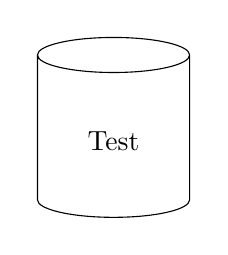
\begin{tikzpicture}
    \node (database) {\drawdatabase{Test}};
  \end{tikzpicture}
  
\begin{tikzpicture}
    \node (document) {\drawdocument{Test}};
  \end{tikzpicture}
  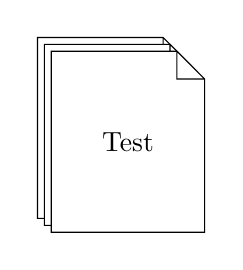
\begin{tikzpicture}
    \node (corpus) {\drawcorpus{Test}};
  \end{tikzpicture}
%%%%%%%%%%%%%%%%%%%%%%%%%%%%%%%%%%%%%%%%%%%%%%%%%%%%%%%%%%%%%%%%%%%%%%%%%%%%%%%%
  \section{Experiments}
\label{sec:experiments}
    We validate the effectiveness of our proposed candidate selection method by using two series of experiments.
    First, we provide a qualitative evaluation of the keyphrase candidates produced by our method and perform a comparison with the other methods.
    Second, we conduct an end-to-end evaluation by exploiting two keyphrase extraction systems.
    
    \subsection{Experimental settings}
    \label{subsec:experimental_settings}
        To quantify the capacity of the candidate selection methods to provide suitable candidates and avoid irrelevant ones, we compute the number of selected candidates (Cand./Doc.) and confront it with the best possible performance (maximum recall~--~R$_{\text{max}}$).
        To do so, we compute a quality ratio (QR):
        \begin{align}
            \text{QR} &= \frac{\text{R$_{\text{max}}$}}{\text{Cand./Doc.}} \times 100
        \end{align}
        The higher is QR, the better.

        \begin{table*}
            \centering
            \begin{tabular}{r|ccc|ccc|ccc}
                \toprule
                \multirow{2}{*}[-2pt]{\textbf{Method}} & \multicolumn{3}{c|}{\textbf{DUC} (\textit{English})} & \multicolumn{3}{c|}{\textbf{SemEval} (\textit{English})} & \multicolumn{3}{c}{\textbf{DEFT} (\textit{French})}\\
                \cline{2-10}
                & Cand./Doc. & R$_{\text{max}}$ & QR & Cand./Doc. & R$_{\text{max}}$ & QR & Cand./Doc. & R$_{\text{max}}$ & QR\\
                \hline
                \{1..3\}-grams & $~~~$596.2 & \textbf{90.8} & 15.2 & 2580.5 & \textbf{72.2} & $~~$2.8 & 4070.2 & \textbf{74.1} & $~~~$1.8\\
                Longest NPs & $~~~$155.6 & 88.7 & 57.0 & $~~~$646.5 & 62.4 & $~~$9.7 & $~~~$914.5 & 61.1 & $~~$6.7\\
                NP-chunks & $~~~$149.9 & 76.0 & 50.7 & $~~~$598.4 & 56.6 & $~~$9.5 & $~~~$812.3 & 63.0 & $~~$7.8\\
                LR-NPs & \textbf{$~~~$143.8} & 85.3 & \textbf{59.3} & \textbf{$~~~$538.2} & 59.4 & \textbf{11.0} & \textbf{$~~~$738.2} & 60.1 & \textbf{$~~$8.1}\\
                \bottomrule
            \end{tabular}
            \caption{Qualitative comparison of the keyphrase candidate selection methods
                     \label{tab:candidate_extraction_statistics}}
        \end{table*}

        \begin{table*}
            \centering
            \resizebox{\linewidth}{!}{
            \begin{tabular}{r@{~}|c@{~~}c@{~~}c@{~}|@{~}c@{~~}c@{~~}c@{~}|@{~}c@{~~}c@{~~}c@{~}|@{~}c@{~~}c@{~~}c@{~}|@{~}c@{~~}c@{~~}c@{~}|@{~}c@{~~}c@{~~}c}
                \toprule
                \multirow{2}{*}[-2pt]{\textbf{Method}} & \multicolumn{6}{c@{~}|@{~}}{\textbf{DUC} (\textit{English})} & \multicolumn{6}{c@{~}|@{~}}{\textbf{SemEval} (\textit{English})} & \multicolumn{6}{c}{\textbf{DEFT} (\textit{French})}\\
                \cline{2-19}
                & \multicolumn{3}{c@{~}|@{~}}{TF-IDF} & \multicolumn{3}{c@{~}|@{~}}{KEA} & \multicolumn{3}{c@{~}|@{~}}{TF-IDF} & \multicolumn{3}{c@{~}|@{~}}{KEA} & \multicolumn{3}{c@{~}|@{~}}{TF-IDF} & \multicolumn{3}{c}{KEA}\\
                \cline{2-19}
                & P & R & F & P & R & F & P & R & F & P & R & F & P & R & F & P & R & F\\
                \hline
                \{1..3\}-grams & 14.3 & 19.0 & 16.1$~~$ & 12.0 & 16.6 & 13.7$~~$ & $~~$9.0 & $~~$6.6 & $~~$7.2$~~$ & 19.4 & 13.7 & 15.9 & $~~$6.7 & 12.5 & $~~$8.6 & 13.4 & 25.3 & 17.3\\
                Longest NPs & 24.2 & 31.7 & 27.0$~~$ & \textbf{14.5} & 19.9 & 16.5$~~$ & 11.7 & $~~$7.9 & $~~$9.3$~~$ & 19.6 & 13.7 & 16.0 & $~~$9.5 & 17.6 & 12.1 & 14.1 & 26.3  &18.1\\
                NP-chunks & 21.1 & 28.1 & 23.8$~~$ & 13.5 & 18.6 & 15.4$~~$ & 11.9 & $~~$8.0 & $~~$9.5$~~$ & 19.5 & 13.7 & 16.0 & $~~$9.6 & 17.9 & 12.3 & 14.3 & 26.8 & 18.4\\
                LR-NPs & \textbf{24.3} & \textbf{32.0} & \textbf{27.2$^\dagger$} & \textbf{14.5} & \textbf{20.0} & \textbf{16.6$^\ddagger$} & \textbf{12.4} & \textbf{$~~$8.4} & \textbf{$~~$9.9$^\ddagger$} & \textbf{20.4} & \textbf{14.4} & \textbf{16.7}& \textbf{10.1} & \textbf{18.5} & \textbf{12.9} & \textbf{14.4} & \textbf{27.0} & \textbf{18.6}\\
                \bottomrule
            \end{tabular}
            }
            \caption{Comparison of TF-IDF and KEA applied on top of different candidate selection methods.
            $\ddagger$ indicates a significant improvement overall candidate sets and $\dagger$ indicates a significant improvement overall candidate sets but the longest NPs at 0.001 level using Student's t-test.
                     \label{tab:keyphrase_extraction_results}}
        \end{table*}
        
        We measure the impact of each candidate selection method on the keyphrase extraction task using the two following unsupervised and supervised keyphrase extraction methods:
        \begin{itemize}
            \item{\textbf{TF-IDF~\cite{jones1972tfidf}:} Word significancy weighting scheme.
                  Words are weighted based on their frequency in the document and the inverse number of documents in which they appear (specificity);
                  Candidates are weighted using the sum of  their words' score.}
            \item{\textbf{KEA~\cite{witten1999kea}:} Naive Bayes classifier trained on two features: the TF-IDF\footnote{KEA computes a TF-IDF based on candidate frequency, whereas our TF-IDF baseline relies on word frequency. KEA's TF-IDF is more efficient on larger documents than smaller ones.} and the first position of each candidate selected within train documents.}
        \end{itemize}
        We report the performance of TF-IDF and KEA in terms of precision~(P), 
        recall~(R) and F1-measure (F) at the top 10 keyphrases.
        Candidate and reference keyphrases are stemmed to reduce the number 
        of mismatches.
    
    \subsection{Candidate selection evaluation}
    \label{subsec:candidate_extraction_evaluation}
        Table~\ref{tab:candidate_extraction_statistics} presents the results of the intrinsic evaluation of the candidate selection methods.
        %Unsurprisingly, the best maximum recall is achieved by the $\{1..3\}$-grams selection method, but at the cost of a huge number of unrelevant candidates as indicated by the low quality ratio.
        Unsurprisingly, the best maximum recall is achieved when selecting $\{1..3\}$-grams, but at the cost of a huge number of irrelevant candidates as indicated by the low QR.
        Among the other selection methods, our method shows a competitive maximum recall while reducing the number of candidates.
        As a consequence, the LR-NPs quality outperforms other selected candidates quality, which is crucial as it directly affects the performance and time complexity of keyphrase extraction methods~\cite{wang2014keyphraseextractionpreprocessing}.
        
        \TODO{examples of true and false positives}
    
    \subsection{Keyphrase extraction evaluation}
    \label{subsec:keyphrase_extraction_evaluation}
        Table~\ref{tab:keyphrase_extraction_results} shows the results of the extrinsic evaluation of the candidate selection methods.
        Overall, we observe that the performance of TF-IDF and KEA is closely correlated with the quality of the set of selected candidates.
        Best results are then obtained when TF-IDF and KEA are applied on LR-NPs (half of them are significantly better).
        Thus, although our proposed selection method does not achieve the best maximum recall, it still outperforms the other candidate selection  methods.
        Comparing longest NPs, NP-chunks and LR-NPs demonstrates that it is efficient to use heuristic based on linguistic properties.

  \section{Conclusion et perspectives}
\label{sec:conclusion_et_perspectives}
  Dans ce travail, nous proposons une méthode à base de graphe pour l'extraction
  non supervisée de termes-clés. Cette méthode groupe les termes-clés candidats
  en sujets, détermine quels sont ceux les plus importants, puis extrait le
  terme-clé candidat qui représente le mieux chacun des sujets les plus
  importants. Cette nouvelle méthode offre plusieurs avantages vis-à-vis des
  précédentes à base de graphe. Le groupement des termes-clés potentiels en
  sujets distincts permet de rassembler des indices utiles auparavant éparpillés
  et le choix d'un seul terme-clé pour représenter un sujet important permet
  d'extraire un ensemble de termes-clés non redondants ( pour $k$ termes-clés
  extraits, exactement $k$ sujets sont couverts). Enfin, le graphe est complet
  et ne requiert plus le paramétrage d'une fenêtre de cooccurrences,
  contrairement aux autres méthodes à base de graphe.

  Les bons résultats de notre méthode montrent la pertinence d'un groupement en
  sujets des candidats pour ensuite les ordonner. Les expériences
  supplémentaires montrent aussi qu'il est encore possible d'améliorer notre
  méthode en proposant une nouvelle stratégie de sélection du terme-clé candidat
  le plus représentatif d'un sujet (pour un gain maximum allant de 4,2 à 15
  points de f-score).

  Nous avons aussi effectué une analyse d'erreurs à partir de laquelle trois
  perspectives de travaux futurs émergent~:

  Nous avons pour objectif d'améliorer la sélection des termes-clés candidats.
  Aussi, des méthodes empruntées à d'autres domaines du TAL peuvent être
  appliquées. Il semble, par exemple, pertinent d'évaluer l'apport des méthodes
  d'extraction terminologiques~\cite{castellvi2001automatictermdetection} pour
  la sélection des termes-clés candidats.
  
  Nous envisageons également d'améliorer le groupement en sujets,
  car celui-ci est très naïf et ne tient compte ni de la synonymie, ni de
  l'ambiguïté des mots. De plus, l'usage du
  radical~\cite{porter1980suffixstripping} des mots n'est pas sans introduire du
  bruit lié à certains faux positifs (p.~ex. \og{}\underline{empir}e\fg{} et
  \og{}\underline{empir}ique\fg{}). L'ajout de connaissances concernant les
  synonymes permettrait de créer des sujets plus complets et une étape de
  désambiguïsation éviterait un groupement systématique des termes-clés
  candidats ayant un ou plusieurs mots en commun. Nous envisageons aussi de
  remplacer la racinisation de \newcite{porter1980suffixstripping} par une
  méthode de lemmatisation. D'un point de vue plus technique, il faudrait
  explorer différentes méthodes de groupement, dont le groupement spectral
  (\textit{spectral clustering}) qui, dans d'autres travaux portant sur
  l'extraction automatique de termes-clés~\cite{liu2009keycluster}, montre de
  meilleures performances que le groupement hiérarchique agglomératif.

  Enfin, une étude détaillée des caractéristiques des termes-clés pourrait
  orienter notre travail vers des critères plus efficaces pour la définition
  d'une stratégie \og{}optimale\fg{} de sélection du terme-clé le plus
  représentatif d'un sujet. Un apprentissage supervisé à partir de certains
  critères est aussi envisagé, au même titre que l'usage de méthodes
  d'optimisation, telles que celle utilisée par
  \newcite{ding2011binaryintegerprogramming} dans leur méthode d'extraction
  automatique de termes-clés.



%  \section*{Acknowledgements}
%  The authors would like to thank the anonymous reviewers for their useful
%  advice and comments. This work was supported by the French National Research
%  Agency (TermITH project -- ANR-12-CORD-0029).

  % include your own bib file like this:
  \bibliographystyle{acl}
  \bibliography{../../biblio}
\end{document}
